%\addcontentsline{toc}{chapter}{Development Process}
\chapter{Design and Experimental Methods}
\section{Design}
The ionic framework for developing mobile hybrid applications encourages the use of the Model View Controller (MVC) compound design pattern. MVC is something which is generally considered good practice within the software engineering industry and therefore the app was designed keeping this in mind.

The model of the app would be the database which is stored on the backend of the system. The view is the html files and the controllers are both the Angular JS controllers and the RESTful PHP API which was created.

\subsection{Overall Architecture}
The overall architecture of the system is complex and involves a lot of different files, this is due to the API having over 35 PHP files where each file performs a specific task. Figure 2.1 shows the overall architecture of the system it doesn't go into each of the specific files however it does provide a good visual representation of the system.

\begin{figure}[H]
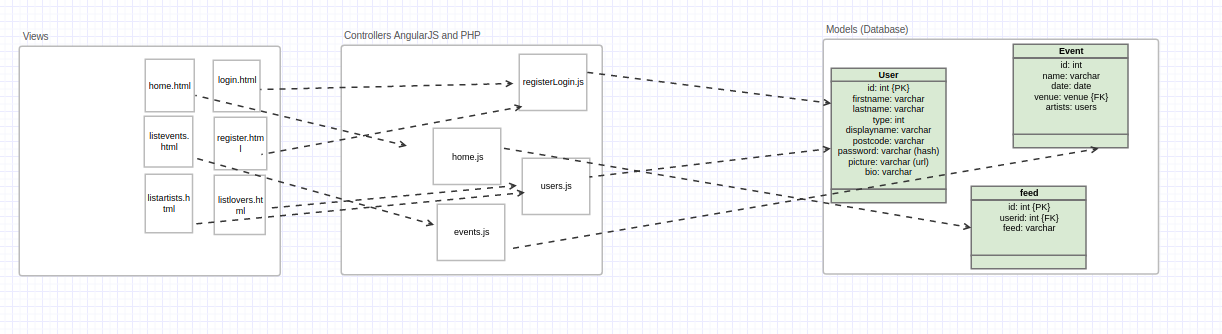
\includegraphics[width=\textwidth,height=\textheight,keepaspectratio]{images/overall}
\caption{Overall architecture of the system.}
\end{figure}

Figure 2.1 shows the system split into the front end view, controllers (which includes both the front end controllers (AngularJS controllers) and the API, PHP file controllers) and the model which is the database. This figure does not show every little detail of the system.

\subsubsection{Use Case Diagram}
Figure 2.2 gives a use case diagram which shows which different features of the app different users can access.

\begin{figure}[H]
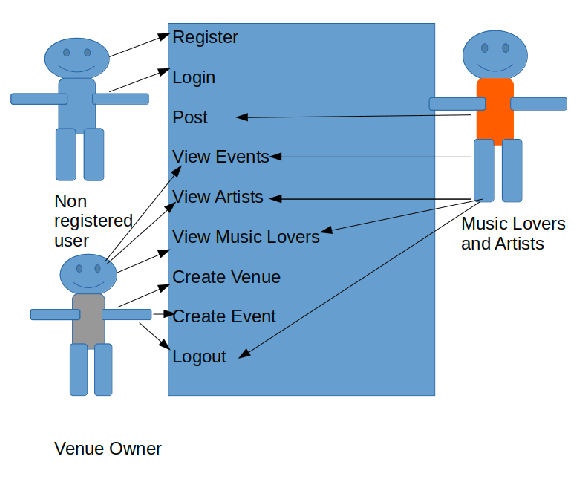
\includegraphics[width=\textwidth,height=\textheight,keepaspectratio]{images/usecase}
\caption{Use case diagram}
\end{figure}



\subsection{Navigation System}
The navigation system is done mainly through view files; a controller is called by the menu. This controller then checks what type of user the logged in user is, if they are a venue owner then it adds more links to the menu. Figure 2.3 (created using \url{https://www.lucidchart.com/}) shows this.

\begin{figure}[H]
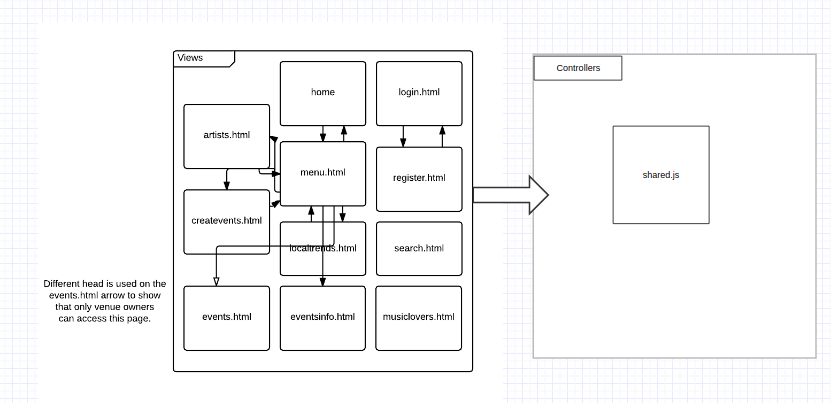
\includegraphics[width=\textwidth,height=\textheight,keepaspectratio]{images/systemdesign}
\caption{UML Diagram which illustrates the view}
\end{figure}

\begin{figure}[H]
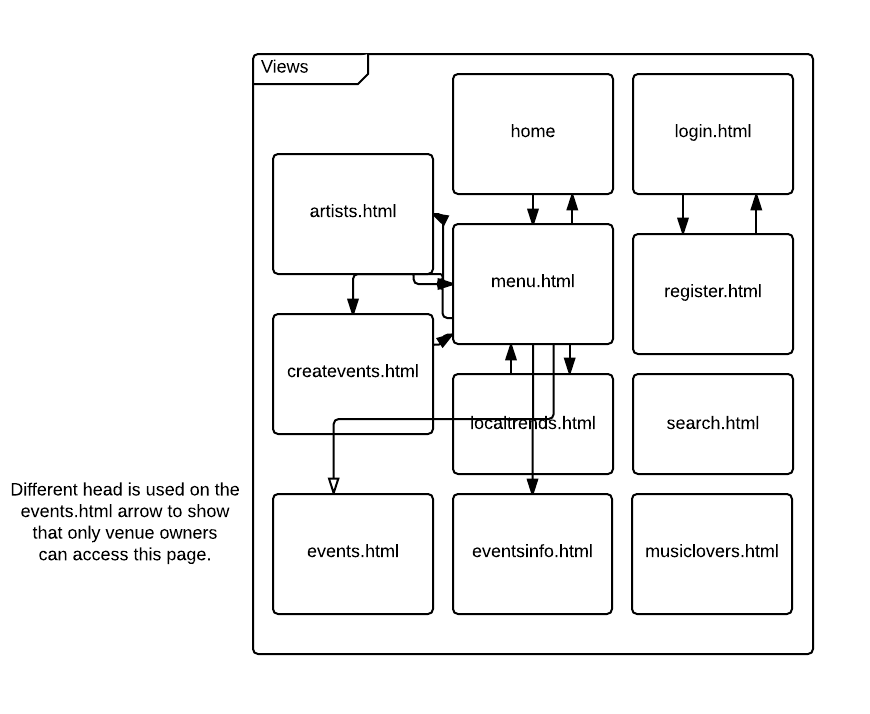
\includegraphics[width=\textwidth,height=\textheight,keepaspectratio]{images/va}
\caption{UML Diagram which illustrates the view interacting with controller.}
\end{figure}
Figure 2.4 shows just the view (created using \url{https://www.lucidchart.com/}) illustrates that once a user has logged in they can access multiple different pages through the menu bar (menu.html). The only page which is restricted is the events.html page as only venue owners can access this page to create events. The register.html page can only be accessed through the login page as it is accessed when a user needs to create a new account to login.

\subsection{Design of registration system}
The design of the registration system considered that there are three different types of user types. The music lovers and artists have the same details whereas venue owners can also create events and venues. Figure 2.5 shows both the UML model for the registration system and the interaction between the model view and controllers. Figure 2.6  contains a flow chart which shows how the login and registration system work when the user launches the app.

\begin{figure}[H]
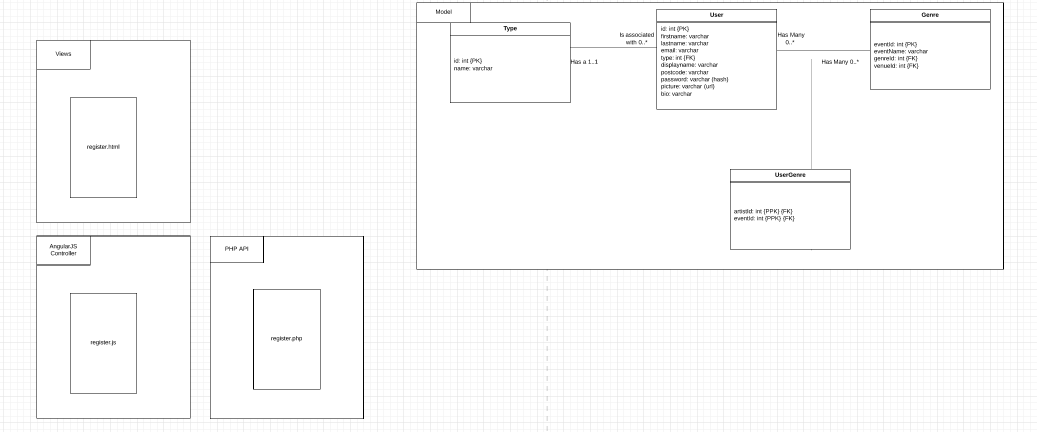
\includegraphics[width=\textwidth,height=\textheight,keepaspectratio]{images/register}
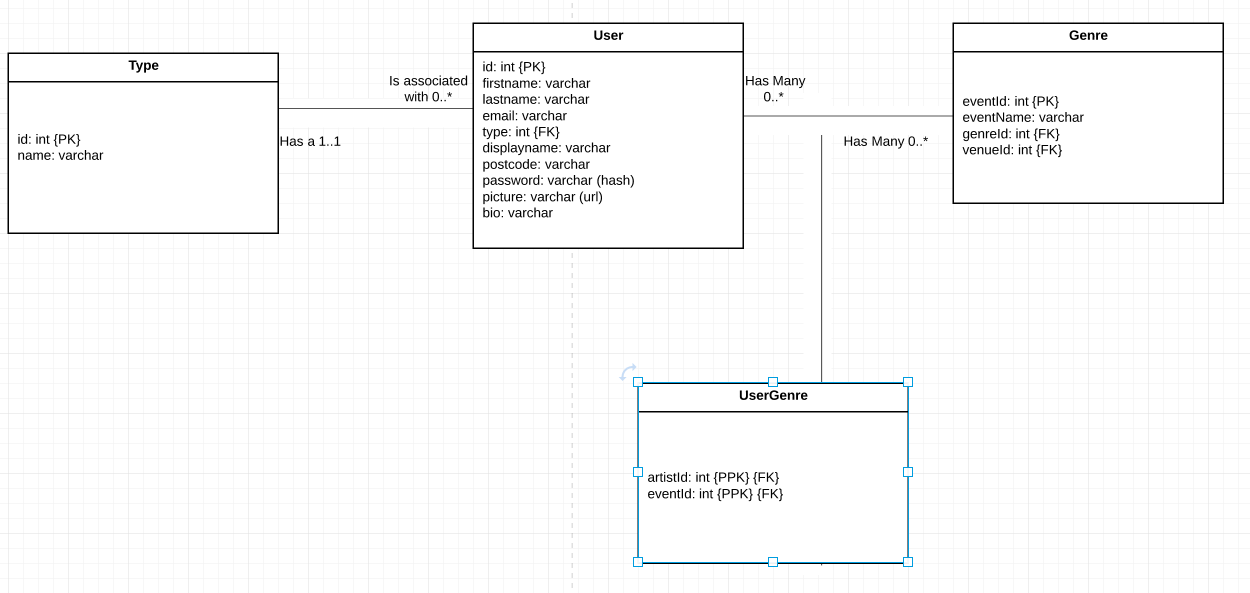
\includegraphics[width=\textwidth,height=\textheight,keepaspectratio]{images/users}
\caption{UML Diagram for the model in relation to a user registering.}
\end{figure}

\begin{figure}[H]
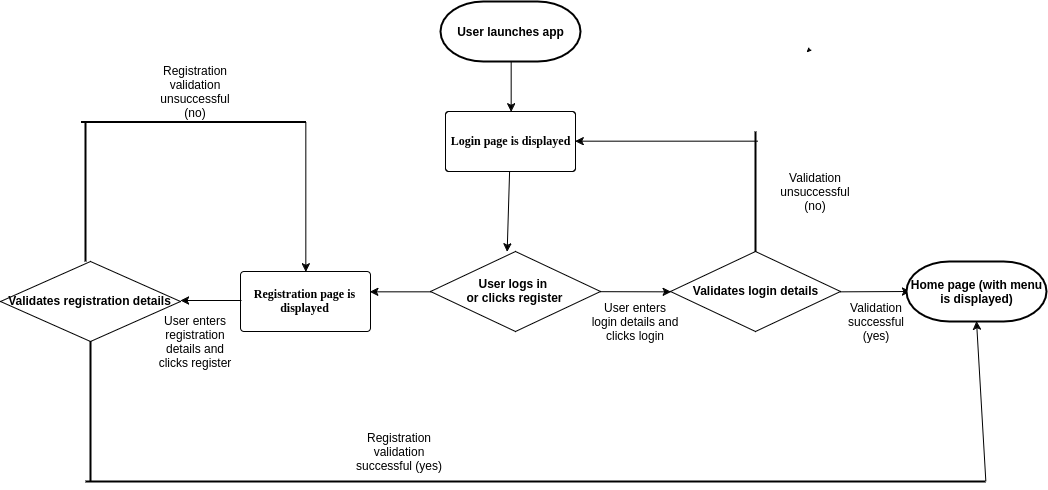
\includegraphics[width=\textwidth,height=\textheight,keepaspectratio]{images/flow}
\caption{Flow diagram for registration system}
\end{figure}



\subsection{Design of events}

Figure 2.7 is a UML diagram (created using \url{Created using https://www.lucidchart.com/}) which shows the appropriate relationships between the different tables in the database in relation to an event. For the interaction with controllers etc. it works in the same way that the registration system does.
\begin{figure}[H]
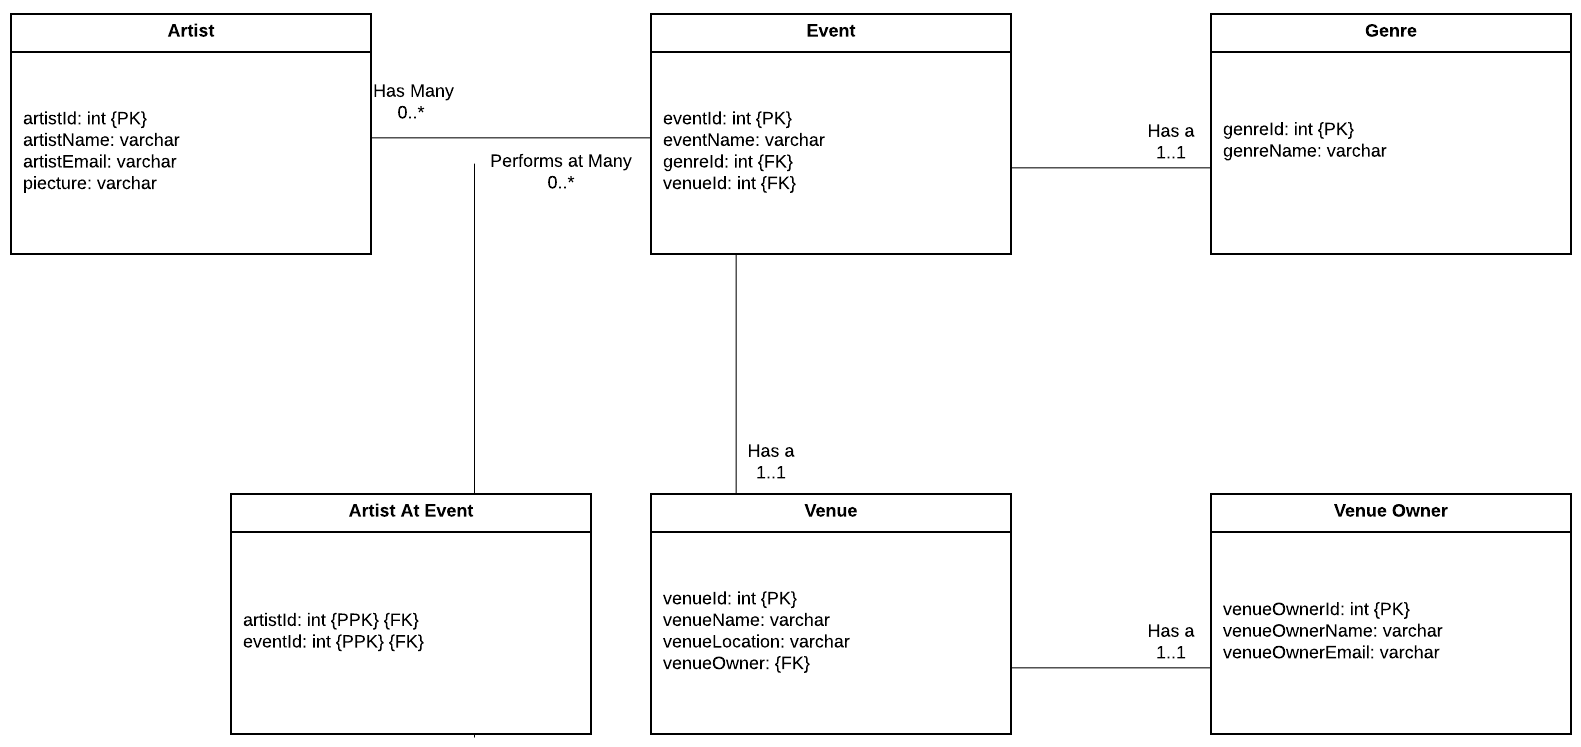
\includegraphics[width=\textwidth,height=\textheight,keepaspectratio]{images/events}
\caption{UML Diagram for the model in relation to events.}
\end{figure}


\subsection{User Interface}
In considering the music social network app, it was decided that the name of the app would be Dynamic. Research into different social media sites was carried out and it was decided that blue would be the main colour used for the app, this is because blue is considered a relaxing colour and in terms of accessibility it is one of the most important colours \cite{col}.
\subsubsection{Shneiderman Principles}
Schniderman came up with eight golden rules for interface design, below the rules are listed followed by how they will be applied to the UI of the app. \cite{sch}
\begin{enumerate}
	\item 'Strive for consistency' - There will be a consistent colour scheme throughout the user interface of the app, along with this navigation (where appropriate) will be the same throughout the app.
	\item 'Enable frequent users to use shortcuts' - There are multiple ways in which this can be applied to a mobile phone app. One way which it will be applied to the app will be allowing the menu (for navigation) to be opened simply by the user swiping the screen to the left. It will also be possible for the user to close the menu by them swiping to the right.
	\item 'Offer informative feedback' - Every time the user clicks a button on the app, the app provides them with feedback in a variety of ways such as by navigating to a different page or by a popup telling them the action they performed was successful.
	\item 'Design dialog to yield closure' - Popups were designed in such a way that the user can is notified of exactly what has happened and thus this will give them closure.
	\item 'Offer simple error handling.' - When things can go wrong for example if the user doesn't have GPS enabled they are informed of what the problem is and what a potential fix for the problem may be.
	\item 'Permit easy reversal of actions.' - The interface was designed so that the user can easily go back and change the options they selected.
	\item 'Support internal locus of control' - The interface has been designed so that the user is fully in control in terms of the data they are submitting and the way they are navigating between different pages.
	\item 'Reduce short-term memory load.' - The only thing which the user must remember is there username and password to access the app.
\end{enumerate}
Figure 2.8 (created using \url {https://www.fluidui.com}) shows some UI mockups which were created. The designs do not show any popup boxes this is because the ionic framework has a default pop up box which uses the device's native popup box.
\begin{figure}[H]
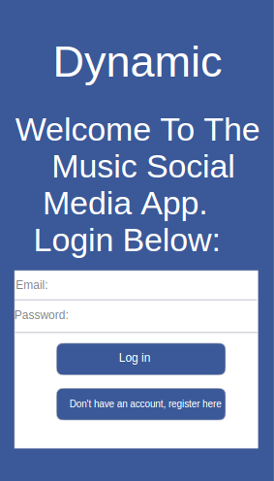
\includegraphics[scale=0.5]{images/ui1}
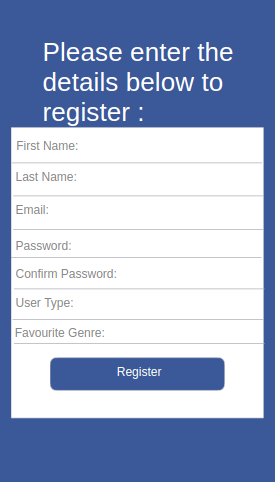
\includegraphics[scale=0.5]{images/ui2}
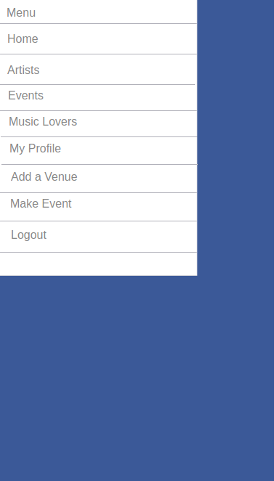
\includegraphics[scale=0.5]{images/ui3}
\caption{User interface mock up}
\end{figure}

\section{Experimental Methods}
As the purpose of the project was to determine whether hybrid apps are feasible alternatives to native apps tests had to be derived. User testing is key to this as it allows for general users (people who use apps on a regular basis) to give feedback about whether they think the hybrid app is as good as a native app, if not why not etc. Another key aspect to answering the question is comparing the resource usage on the device of the hybrid app to a standard app, this will include comparing things such as amount of RAM being used.

Finally, during each story in the development process, it was considered whether using hybrid app technology was as challenging, more challenging or less challenging than developing using native app technologies.

\subsection{User Testing}
In establishing whether hybrid apps are feasible alternatives to native apps it was important to get general users thoughts about the app which had been produced. Within the development community there is a bit of a stigma associated towards hybrid mobile applications therefore to remove bias the majority of people who fill in the questionnaires associated with the app will be lay people.

Whilst clearly it would be great to get many people to participate by filling in a questionnaire realistically only around 10 people were chosen. Before asking each individual question, the project was explained to them.

The following questions were asked to everyone who participated (a blank copy of the questions asked is in  Appendix 4.)

\begin{enumerate}
\item On a scale of 1 to 10, with 1 being slowest and 10 being very fast in your opinion how quick is the app at processing the registration form?
\item On a scale of 1 to 10 with 1 being significantly slower than a native app 5 being about the same time as a native app and 10 being significantly faster than a native app. In your opinion, how quick is the app at processing the registration form?
\item On a scale of 1 to 10 with 1 being slowest and 10 being fast in your opinion how long does the process of uploading a profile picture take?
\item On a scale of 1 to 10 with 1 being significantly slower than a native app, 5 being about the same and 10 being very fast, faster than a native app. In your opinion how long does the process of uploading a new profile picture take?
\item On a scale of 1 to 10 with 1 being slowest and 10 being fast in your opinion how long does the process of viewing events and sorting them by using nearest events (GPS) take?
\item On a scale of 1 to 10 with 1 being significantly slower than a native app, 5 being about the same as a native app and 10 being very fast, faster than a native app in your opinion how long does the viewing events and sorting them by using nearest events (GPS) take?
\end{enumerate}
These questions were decided upon as they ensured that all of the stories which were relevant in terms of testing different elements of hybrid technologies can be tested.
